\documentclass{beamer}
\usepackage[latin1]{inputenc}
\usetheme{Goettingen}
\title{Multiprocessor Scheduling with the Aid of Network Flow Algorithms}
\author{Harold S. Stone}
\institute{Member, IEEE}
\date{Jan, 1977}
\begin{document}

\begin{frame}
\titlepage
\end{frame}

%Outline-----------------------------------------------------------------------------------------------------
\section{Overview}

\begin{frame}{Problem}
\begin{itemize}
	\item \cite{sto77}
	\item Assignment of computational units
	\item 2 processor systems
	\item Distributed (ARPANET)
\end{itemize}
\end{frame}

\begin{frame}{Solution}
\begin{itemize}
	\item Use max flow/min cut to assign computational units
	\item Some units float between processors during execution
	\item Monitor working set to decide when to swap units
	\item Static analysis of costs and problem to determina optimal assignment pre-execution
\end{itemize}
\end{frame}

%Outline-----------------------------------------------------------------------------------------------------
\section{Background}

\begin{frame}{Assignment}
\begin{itemize}
	\item Minimize ``cost''
	\begin{itemize}
		\item Execution time
		\item Communication time
		\item (reassignment time)
		\item (coordination overhead)
	\end{itemize}
	\item Simultaneous objectives with common currency
\end{itemize}
\end{frame}

\begin{frame}{Dynamic and Static}
\begin{itemize}
	\item Assign processes optimally
	\item Dynamically reassign during runtime
	\item Information unavailable at compile time?
	\item Assignment stages?
\end{itemize}
\end{frame}

\begin{frame}{Floating units}
\begin{itemize}
	\item ``permitted to {\em float} from processor to processor during execution''
	\item Is this actually useful?
	\item Multiple copies?
\end{itemize}
\end{frame}

\begin{frame}{Exploiting locality}
\begin{itemize}
	\item Communication incurrs reatively high overhead
	\item Distributed memory
	\item Possibly different computational speeds (gpgpu's, CPUs)
\end{itemize}
\end{frame}

\begin{frame}{2 processor system}
\begin{itemize}
	\item Distributed
	\item Heterogeneous
	\item System 360 + microprogrammable minicomputer \cite{sta74}
	\item Limitation?
\end{itemize}
\end{frame}

\begin{frame}{C.mmp}
\begin{itemize}
	\item Interconnection network \cite{wul72}
	\item 16 processors (homogeneous)
	\item 16 Memories
	\item Shared Crossbar
	\item Shared memory system?
\end{itemize}
\end{frame}

\begin{frame}{Implications}
\begin{itemize}
	\item Presumes serialisability
	\item Presumes data independance
	\item Dependancies among communication cost and assignment?
\end{itemize}
\end{frame}

%Cutsets-----------------------------------------------------------------------------------------------------
\section{Solution}

\begin{frame}{Minflow Maxcut}
\begin{columns}
\begin{column}{5cm}
\begin{itemize}
	\item Ford Fulkerson
	\item while there exists an unsaturated path from s to t, saturate it
	\item Edmonds Karp, $O(n^5)$ : $O(VE^2)$
	\item Duality
\end{itemize}
\end{column}
\begin{column}{5cm}
\center{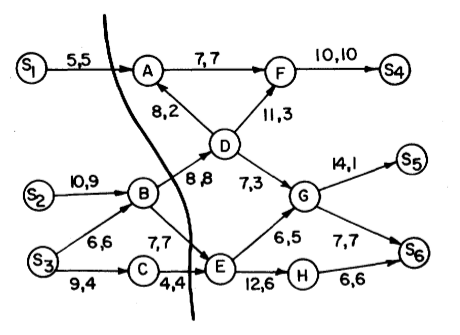
\includegraphics[width=5cm]{../res/maxflow.png}}
\end{column}
\end{columns}
\end{frame}

\begin{frame}{Commodity Flow}
\begin{itemize}
	\item Abstraction of computation
	\item Computational graphs (SDF)
	\item Data flowing between computational units
\end{itemize}
\end{frame}

\begin{frame}{Representing}
\begin{columns}
\begin{column}{5cm}
\begin{itemize}
	\item computational units as vertices
	\item communication cost as edges
	\item add 2 vertices a and b as the 2 processors
	\item Add 2 edges from every vertex to every other vertex
	\begin{itemize}
		\item (x,b) edge, cost of assigning to a
		\item (x,a) edge, cost of assigning to b
	\end{itemize}
	\item Min ab cut is cost of minimal assignment
\end{itemize}
\end{column}
\begin{column}{5cm}
\center{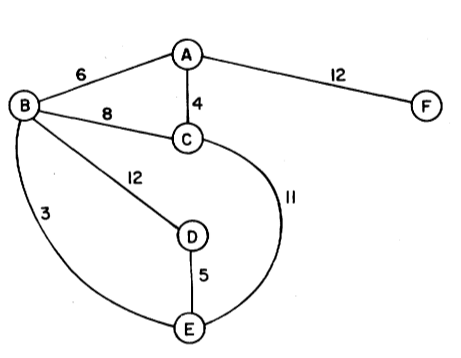
\includegraphics[width=5cm]{../res/intermodule.png}}
\end{column}
\end{columns}
\end{frame}

\begin{frame}{Correctness}
\begin{columns}
\begin{column}{4cm}
\begin{itemize}
	\item cut must separate all vertices from 1 of the ``source'' or ``sink'' nodes
	\item cut separates some processors along communication
	\item These are the parts of the module assignment cost
\end{itemize}
\end{column}
\begin{column}{6cm}
\center{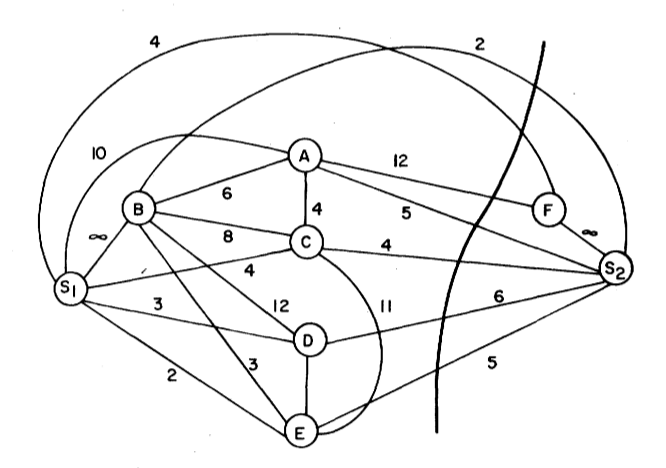
\includegraphics[width=6cm]{../res/mincut.png}}
\end{column}
\end{columns}
\end{frame}

\begin{frame}{Dynamic}
\begin{itemize}
	\item Reassign during execution
	\item recompute assignment, known quantities shouldnt change
	\item Does data change?
	\item Is data unknowable at execution time?
\end{itemize}
\end{frame}

\begin{frame}{In Practice}
\begin{itemize}
	\item Not practical to force user to supply data
	\item Must be determined on fly in real time
	\item Change in working set - monitor
	\item Actual implementation (Michael and Burns), too early to say how useful
\end{itemize}
\end{frame}

\begin{frame}{Importance}
\begin{itemize}
	\item Allows to generalise to n processors
	\item 2 processors only constant speedup :)
	\item (nowdays) required for parallelism, model presumes serialisability
\end{itemize}
\end{frame}

\begin{frame}{Representation}
\begin{columns}
\begin{column}{5cm}
\begin{itemize}
	\item Similar as above, add a new vertex for each processor
	\item Edge from node to processor has cost weighted average of other nodes minus this node
	\item Negative edges, can linearly increase all edges so no edge is negative
	\item no proof :(
\end{itemize}
\end{column}
\begin{column}{5cm}
\center{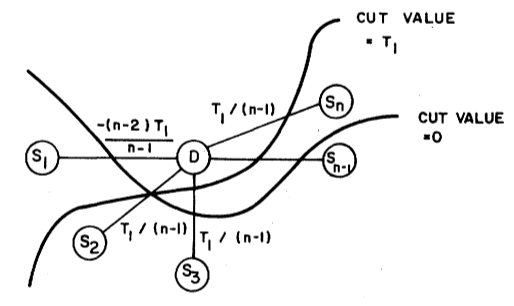
\includegraphics[width=5cm]{../res/multicut.png}}
\end{column}
\end{columns}
\end{frame}

\begin{frame}{Complexity}
\begin{itemize}
	\item We call this NP Hard
	\item Several iterations of 2-processor assignment, perform 2 assign for every pair of processors, $O(n^{10})$
	\item We can presume this is not correct, NP
	\item Complexity of problem?
\end{itemize}
\end{frame}

%Impact-----------------------------------------------------------------------------------------------------
\section{Discussion}

\begin{frame}{Dynamic Assignment}
\begin{itemize}
	\item Cloud computing
	\item We never really do this mid-execution
	\item ``semi-dynamic'' module assignment
\end{itemize}
\end{frame}

\begin{frame}{Cost model}
\begin{itemize}
	\item Implicitly serial execution
	\item Combines multiple goals of system
	\item Must generalise for variable communication cost
	\item Must generalise for assignment-dependant cost
\end{itemize}
\end{frame}

\begin{frame}{Locality}
\begin{itemize}
	\item This one is important
	\item Mapreduce
	\item Less about dynamic reassignment
	\item Static knowledge of processing requirements?
\end{itemize}
\end{frame}

\begin{frame}{Research Questions}
\begin{itemize}
	\item Splitting hairs: Power usage?
	\item Simultaneous execution: My work
	\item Accounting for module reassignment: We dont. Is this even possible?
\end{itemize}
\end{frame}

%TIDYING UP-----------------------------------------------------------------------------------------------------
\section{Questions}
\begin{frame}[allowframebreaks]{References}
\bibliographystyle{wmaainf}
\bibliography{biblio}
\end{frame}

\begin{frame}{Questions?}
\end{frame}

\end{document}